% Uncomment one of three below
%\RequirePackage[]{optional}
\RequirePackage[notslides]{optional}
%\RequirePackage[slides]{optional}

\opt{slides}{
% Following for presentation mode
\documentclass[10pt]{beamer}
\usepackage{xmpmulti}
%usetheme{Berlin}
}
\opt{notslides}{
% Following for notes mode
\documentclass[a4paper]{article}
\usepackage{beamerarticle}
\usepackage{a4wide}
\usepackage{graphicx}
\usepackage{amsfonts}
\usepackage{fancyhdr}
}

% Following for all modes
%\usepackage{auto-pst-pdf}
%\usepackage{pst-pdf}
\usepackage{psfrag}

\parindent=0ex
\parskip=1ex
\newcommand{\conv}{\ast}
\reversemarginpar

%\title{Systems}
%\author{}
%\date{}

\begin{document}
\pagestyle{fancy}
\fancyhead{}
\renewcommand{\headrulewidth}{0pt}
\fancyfoot[C]{\thesection-\thepage}
%\fancyfoot[R]{fcn2010}

\begin{frame}
  \titlepage
\end{frame}

\setcounter{section}{2}
\section{Systems}

%\mode<article>{{\bf \LARGE Systems} \newline}

%\fbox{
%  \begin{minipage}{0.97\textwidth}
%    \tableofcontents
%  \end{minipage}
%}

In its simplest form, a system is a mathematical transformation that acts on an input signal to produce an output signal.  We depict a system in block diagram form as follows:
\begin{center}
  \psfrag{x(t)}{\scriptsize $x(t)$}
  \psfrag{y(t)}{\scriptsize $y(t)$}
  \psfrag{y(t)=T{x(t)}}{\scriptsize $y(t)=T\{x(t)\}$}
  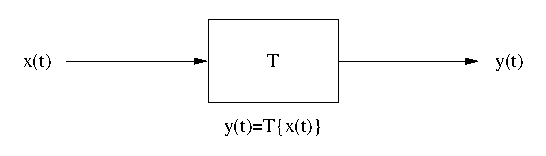
\includegraphics{simplesystem}
\end{center}
Associated with every system is an input-output relation, or recipe, expressed above in the form $y(t) = T\{x(t)\}$.  For any given input $x(t)$, this recipe lets you find the corresponding output signal $y(t)$.  Different systems obviously have different input-output relations, and in general two different systems will produce a different output for the same input.

We've already encountered two examples of systems, without directly thinking about them in this formal context.  At the end of the previous section we considered two signals $x(t)$ and $y(t)$ linked by the differentiation property:  $y(t) = \frac{d}{dt} x(t)$.  This has a system-level interpretation:  consider a system called a {\em differentiator}, which takes a signal $x(t)$ at the input, produces a signal $y(t)$ at the output, and with the input-output recipe $y(t) = T\{x(t)\} = \frac{d}{dt} x(t)$:
\begin{center}
  \psfrag{x(t)}{\scriptsize $x(t)$}
  \psfrag{y(t)}{\scriptsize $y(t)$}
  \psfrag{y(t)=d/dtx(t)}{\scriptsize $y(t)=\frac{d}{dt} x(t)$}
  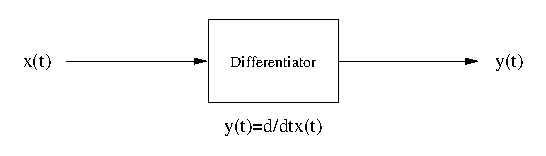
\includegraphics{differentiatorsystem}
\end{center}
If I tell you that the input signal to this system is $x(t) = \sin(\omega_0 t)$, then you can use the input-output relation to find the corresponding output:
\begin{equation*}
  y(t) = T\{x(t)\} = \frac{d}{dt} \{x(t)\} = \frac{d}{dt} \sin(\omega_0 t) = \omega_0 \cos(\omega_0 t).
\end{equation*}
If the input signal is $x(t) = u(t)$, then the output is
\begin{equation*}
  y(t) = T\{x(t)\} = \frac{d}{dt} \{x(t)\} = \frac{d}{dt} u(t) =\delta(t).
\end{equation*}
The recipe that governs the action of the system therefore lets you calculate the output for any given input.

An integrator system can also be defined by means of an input-output relation:
\begin{center}
  \psfrag{x(t)}{\scriptsize $x(t)$}
  \psfrag{y(t)}{\scriptsize $y(t)$}
  \psfrag{y(t)=intx(t)}{\scriptsize $y(t)=\int_{-\infty}^t  x(\tau) d\tau$}
  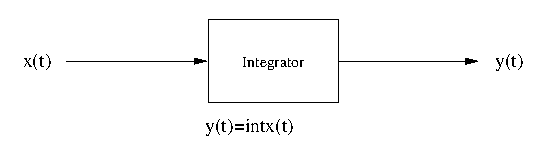
\includegraphics{integratorsystem}
\end{center}
Again, for any input $x(t)$ you can use the input-output recipe for the system to find the corresponding output.  For example, if the input is $x(t) = \delta(t)$ then the output must be
\begin{equation*}
  y(t) = T\{x(t)\} = \int_{-\infty}^t x(\tau) d\tau = \int_{-\infty}^t \delta(\tau) d\tau = u(t).
\end{equation*}
Alternatively, if the input is $x(t) = p_1(t)$ then the output must satisfy
\begin{equation*}
  y(t) = T\{x(t)\} = \int_{-\infty}^t x(\tau) d\tau = \int_{-\infty}^t p_1(\tau) d\tau,
\end{equation*}
which can be evaluated and plotted as follows:
\begin{center}
  \psfrag{t}{\scriptsize $t$}
  \psfrag{y(t)}{\scriptsize $y(t)$}
  \psfrag{1/2}{\scriptsize $\frac{1}{2}$}
  \psfrag{-1/2}{\scriptsize $-\frac{1}{2}$}
  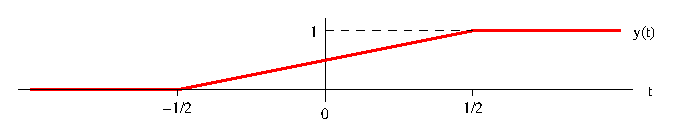
\includegraphics{intpulsesig}
\end{center}

It is really important to understand that an integrator takes a signal at the input and produces {\em a signal} at the output.  This is due to the presence of the time variable $t$ as the upper limit of the integral:  for every value of $t$ the limits of the integral changes, and so does the value of the integral.  Most students, when asked "What is the inverse operation of differentiation?" will answer "Integration".  {\em This is not correct.}  The inverse of differentiation is {\em indefinite integration}.  Indefinite integration, when applied to a function, produces another function, while (in the usual sense) when you integrate a function you get a value.  The difference is critical.

We can also string systems together.  The system
\begin{center}
  \psfrag{x(t)}{\scriptsize $x(t)$}
  \psfrag{y(t)}{\scriptsize $y(t)$}
  \psfrag{z(t)}{\scriptsize $z(t)$}
  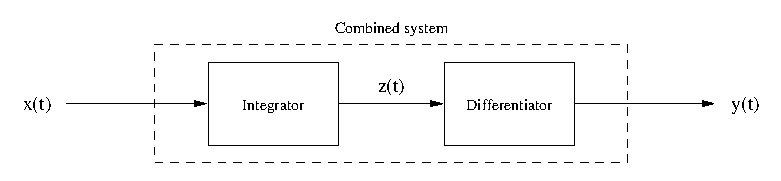
\includegraphics{intdiffsystem}
\end{center}
as two components, and we can trace the signals through:  $z(t) = \int_{-\infty}^t x(\tau) d\tau$ and $y(t) = \frac{d}{dt} z(t)$.  Since integration and indefinite integration are inverses of one another, this means that $y(t) = x(t)$.  Considered as a whole, we can therefore think of this as a combined system with input $x(t)$ and output $y(t)$.  The input-output relation for this combined system is $y(t) = T\{x(t)\} = x(t)$, which produces at the output exactly the same signal as appeared at the input.

\subsection{Differential equations as input-output relations}

We can use the notion of a system to represent the relationship between signals in a physical setting.  For example, the circuit below contains a current source driving a parallel combination of a resistor and a capacitor:
\begin{center}
  \psfrag{x(t)=i(t)}{\scriptsize $x(t)=i(t)$}
  \psfrag{iC(t)=y(t)}{\scriptsize $i_C(t)=y(t)$}
  \psfrag{iR(t)}{\scriptsize $i_R(t)$}
  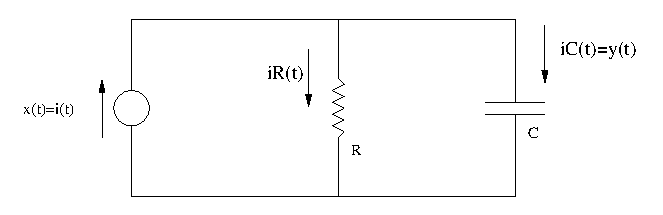
\includegraphics{circuitrcparallel}
\end{center}
Suppose we are interested in the signal corresponding to the current through the capacitor as we change the current produced by the source.  These are functions of time, and can be thought of as signals.  In this case we can think of the circuit as a system:  the input $x(t)$ is the input current $i(t)$, and the output $y(t)$ is the capacitor current $i_C(t)$.  The laws of physics (expressed as the theory of electrical circuits) let us find the output signal for any given input signal.

The voltage-current relationship for a resistor can be expressed in terms of signals as $v(t) = R i_R(t)$, and the relationship for a capacitor is $i_C(t) = C \frac{d}{dt} v(t)$.  Note that the voltage signal across the two circuit elements is equal, and is given by $v(t)$.  We can eliminate $v(t)$ from these expressions, yielding $i_C(t) = R C \frac{d}{dt} i_R(t)$.  However, we know that $i_R(t) = i(t) - i_C(t)$, so $i_C(t) = R C \frac{d}{dt} (i(t) - i_C(t))$.  This provides a relationship between $i(t)$ and $i_C(t)$:
\begin{equation*}
  i_C(t) + RC \frac{d}{dt} i_C(t) = RC \frac{d}{dt} i(t).
\end{equation*}
Using our definitions of input and output signals, the input and output of the system must obey the relation
\begin{equation*}
  y(t) + RC \frac{d}{dt} y(t) = RC \frac{d}{dt} x(t).
\end{equation*}
This is just a recipe for finding the output signal for any given input signal, which is all that is required to specify a system.  If I tell you that the input is $x(t) = u(t)$, then you know that the output must satisfy
\begin{equation*}
  y(t) + RC \frac{d}{dt} y(t) = RC \frac{d}{dt} u(t),
\end{equation*}
which is just a differential equation with one unknown $y(t)$.  Assuming you know how to solve differential equations, you could solve for the output as $y(t) = e^{-\frac{1}{RC}t} u(t)$, which for $RC=1$ is shown below:
\begin{center}
  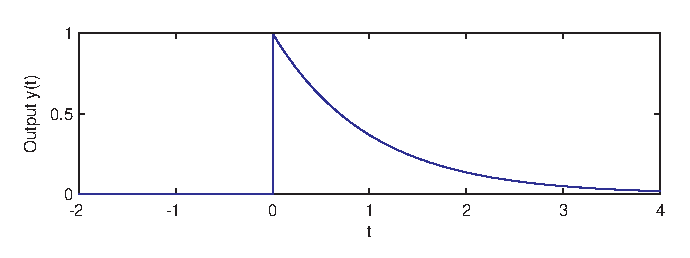
\includegraphics{circuitrcparstepresp}
\end{center}
After the step the current initially all flows through the capacitor, which begins charging.  Once charged, all the current flows through the resistor so the output signal goes to zero.

There is one subtlety in this example.  The input-output relation for the system just described is a first-order differential equation in the output $y(t)$, so the solution is only defined up to a single unknown integration constant.  An auxiliary condition is required in order to specify the output $y(t)$ uniquely for a given input $x(t)$.  In the description given above the initial condition was that prior to $t=0$ the capacitor held no charge --- this is often called the {\em initial rest condition}.  At this stage we do not concern ourselves with the technical details.

The power of thinking at a system level comes from abstraction.  Once you (or somebody else) have done the physical modelling it no longer matters that the system represents an electrical circuit.  You have a mathematical model, expressed in terms of an input-output relation, which for all practical purposes {\em replaces} the physical system with a mathematical representation.  Thus you can work with signals and systems without having to think about details that are irrelevant to solving the problem.

\subsection{System properties}
The most general form for an input-output relation for a system is $y(t) = T\{x(t)\}$.  This expression indicates that the system is characterised by a transformation $T\{\cdot\}$, which acts on the input to produce the output.  

It usually makes things much clearer if you think about a signal as an {\em object}, rather than as a set of values of a function for different instants in time.  The expression $y(t) = T\{x(t)\}$ can then be interpreted as follows:  the system takes the object $x(t)$, applies the transformation $T$ to it, to produce the object $y(t)$.  

You've seen this way of thinking with vectors and matrices.  If I were to say that $\mathbf{x}$ and $\mathbf{y}$ were vectors (say in $\mathbb{R}^n$), and that they are linked by the matrix $\mathbf{A}$ in the relation $\mathbf{y} = T\{\mathbf{x}\} = \mathbf{A} \mathbf{x}$, this would be the natural interpretation.  The transformation $T$ is now represented by the matrix $\mathbf{A}$, which acts on the object $\mathbf{x}$ to produce the object $\mathbf{y}$ by matrix-vector multiplication.  In reality the objects $\mathbf{x}$ and $\mathbf{y}$ are (ordered) collections of numbers, but as far as the structure of transformations is concerned this fact is not particularly useful.  Exactly the same is true for signals\footnote{This is more true than it might appear.  The abstract mathematical construct of a {\em vector space} is entirely appropriate for signals and systems:  the structure of the mathematics on "ordinary" vectors is exactly the same as the structure of the mathematics for signals.  In this context a function (or a signal) $x(t)$ {\em is a vector}, and it really does no harm thinking of it as such.}.

In practice the general transformation $y(t) = T\{x(t)\}$ is not particularly useful:  the set of {\em all} possible transformations that can be applied to $x(t)$ to produce $y(t)$ is too big to permit a useful mathematical theory.  We therefore have to restrict the set of possible transformations that we consider, and this corresponds to making assumptions about the properties of the systems that they represent.

\subsubsection{Causal systems}

In the real world, physical systems always exhibit a property called causality:  the state of an object can only depend on things that happened to it {\em in the past}.  A soccer ball cannot know that somebody is going to kick it tomorrow, so its position today can't in any way depend on what is going to happen to it in the future.  Put another way, the {\em cause} of something always precedes the {\em effect}.  

Suppose I think of the soccer ball as a system, and assume that it is only free to move in a straight line.  I can put a coordinate system down along this straight line (with an arbitrary origin), and at any instant in time I can express the position of the ball with respect to this coordinate system.  The position of the ball at any time can be expressed by the value of a function $y(t)$ at that instant.  The signal $y(t)$ then represents the position of the ball at every possible time instant, and I consider this to be the output of the system.  The input $x(t)$ is the force that I apply to the ball, in the direction that it is free to move, expressed as a function of time.  Clearly we now have a physically-realisable system, where the input signal is the force applied to the ball and the output is its position.  Using Newton's laws of motion I could derive a relationship linking input to output.

I could certainly drive this system with the input signal $x(t) = u(t)$, which contains a step change in the force applied at time $t=0$.  But what do we mean by $t=0$?  And what do we mean by negative time?  The answer is that, as was the case with the position axis before, we can put the origin anywhere we like --- but once we've fixed what we consider to be $t=0$ then this is the time origin for {\em all} our signals.  I could, for example, define time $t=0$ to be "now!", in which case yesterday would be on the negative time axis and tomorrow would be on the positive axis (as long as I put the positive time direction going into the future, which is the convention).

Returning to the soccer ball example with $x(t) = u(t)$, I denote by $t=0$ the instant at which I start applying the force.  For all time prior to $t=0$, no force has ever been applied to the ball.  It is reasonable, therefore, to assume {\em initial rest conditions} for the ball --- it carries no energy and isn't moving.  For simplicity we may as well place the (arbitrary) origin of the position axis at the position of the ball for negative time --- in this case we would have $y(t) = 0$ for $t<0$.  However, as soon as the force is applied the ball starts moving, so we would be quite satisfied if someone told us that an input-output pair for the system looked as follows:
\begin{center}
  \psfrag{t}{\scriptsize $t$}
  \psfrag{x(t)}{\scriptsize $x(t)$}
  \psfrag{y(t)}{\scriptsize $y(t)$}
  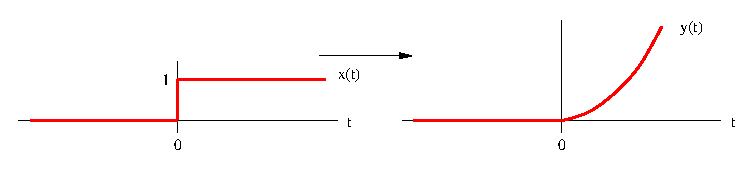
\includegraphics{causalballpair}
\end{center}

But what if someone told you that the input-output pair was
\begin{center}
  \psfrag{t}{\scriptsize $t$}
  \psfrag{x(t)}{\scriptsize $x(t)$}
  \psfrag{y(t)}{\scriptsize $y(t)$}
  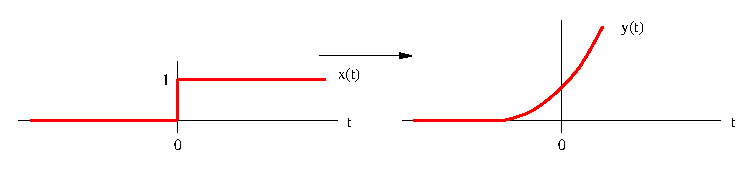
\includegraphics{causalballpair2}
\end{center}
This would not be plausible --- the ball started moving (the effect) before the force was applied (the cause).  The response in the second case couldn't be the output of a causal system.

Since the behaviour of a system is determined by its input-output relation, it must be possible to examine this relation in order to determine if the system is causal.  The easiest way of doing this is to fix a value of $t$, say $t = t_0$, and think about calculating the output value $y(t_0)$ using the input-output relation.  Ask yourself:  "In order to find the value of $y(t_0)$, what values of the input $x(t)$ do I need to know?"  This answer defines a set of values of $t$ for which you need to know $x(t)$.  If you only need to know $x(t)$ at instants in time that occur {\em earlier} than $t=t_0$, then causality is indicated.  In practice you need to ask this question for {\em every} possible value of $t_0$ in order to prove causality.

Here's an example.  Suppose the input-output relation for a system is given by
\begin{equation*}
  y(t) = \int_{-1}^1 x(t - \tau) d\tau.
\end{equation*}
Is it causal?  To get some insight, consider finding $y(0) = \left. y(t) \right|_{t=0}$.  According to the input-output relation, $y(0) = \int_{-1}^1 x(0 - \tau) d\tau = \int_{-1}^1 x(- \tau) d\tau = \int_{-1}^1 x(p) dp$.  To calculate this integral we need to know $x(t)$ over the entire integration interval $[-1, 1]$.  This interval includes instants later than $t=0$.  Thus the system is not causal.

Is the system represented by the input-output relation
\begin{equation*}
  y(t) = \int_{0}^1 x(t - \tau) d\tau
\end{equation*}
causal?  In this case $y(0) = \int_{0}^1 x(0 - \tau) d\tau$, so we need to know $x(-\tau)$ over the interval $[0, 1]$.  Equivalently, we need to know $x(t)$ over the interval $[-1, 0]$, all of which are in the past.  For $t=0$, at least, the system is exhibiting the required condition for causality.  To prove that it for all values of $t$, do the change of variables $p = t - \tau$, where $t$ is a constant in the integration.  The input-output relation is then 
\begin{equation*}
  y(t) = \int_{t-1}^t x(p) dp.
\end{equation*}
Clearly, to find the value of the output at time $t$ we need to know the values of the input over the interval $[t-1, t]$, and none of these inputs are in the future.  The system is therefore causal.

Causality is a property of physical systems, and if we construct models of such systems then it is sensible to require that the models are causal.  However, the mathematical theory of signals and systems doesn't really differentiate between models that are causal and those that are not:  working with a causal system isn't really any easier than working with a non-causal system.  There are other properties that a system can have for which this is absolutely not the case:  certain systems have properties that make it {\em much} easier to work with them.  The remainder of this section discusses some of these properties.

Finally, it is worth noting that while causality is important in modelling a physical system, non-causal systems are both important and useful.  Suppose someone gives you a DVD full of data obtained by sampling the swell size of the ocean in False Bay over a period of 100 years, and you want to process this data to highlight important events.  You could design a system (or a filter) that takes this data as an input $x(t)$, and transforms it to an output $y(t)$ that is more informative for your purposes.  There's no good reason to require that the system you design be causal --- all the data is available, and it could do a better filtering job if the output at any point depended on input values that are both in the future and the past relative to that point.  Another example is in image processing:  in an image there is no time axis, so causality has no meaning and no relevance.

\subsubsection{Linear systems}

Let $f(x)$ be a real-valued function, and let $x$ and $y$ be real-valued variables:  $f$ is homogeneous if for any constant $a$ we have $f(ax) = af(x)$ for all $x$, and $f$ is additive if $f(x+y) = f(x) + f(y)$ for all $x$ and $y$.  If these two properties hold then the function $f$ is said to be linear, and for any constants $a$ and $b$ it must be true that $f(a x + b y) = a f(x) + b f(y)$ for all $x$ and $y$.  Clearly a linear function is a very restricted form.

Systems can also be linear, and the requirements are similar to those just outlined for functions.  A linear system has a very particular structure, and behaves nicely with regard to sums and scalings of signals.  Systems that are linear have very tractable mathematics.

Consider again the canonical system
\begin{center}
  \psfrag{x(t)}{\scriptsize $x(t)$}
  \psfrag{y(t)}{\scriptsize $y(t)$}
  \psfrag{y(t)=T{x(t)}}{\scriptsize $y(t)=T\{x(t)\}$}
  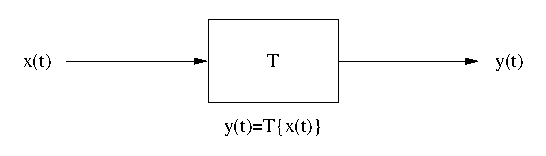
\includegraphics{simplesystem}
\end{center}
Homogeneity and additivity (and therefore linearity) of the system are related to the behaviour of the transformation $T$.  If $T\{a x(t)\} = a T\{x(t)\}$ for all signals $x(t)$ and any constant $a$, then the system is homogeneous.  If $T\{x(t) + y(t)\} = T\{x(t)\} + T\{y(t)\}$ for all signals $x(t)$ and $y(t)$, then the system is additive.  The system is linear if it is both additive and homogeneous, in which case for any constants $a$ and $b$ we must have $T\{a x(t) + b y(t)\} = a T\{x(t)\} + b T\{y(t)\}$ for all signals $x(t)$ and $y(t)$.

These statements are cryptic --- what do they mean?  Let's consider a system that is homogeneous, and consider driving it with the input signal $x(t) = x_1(t)$.  The output will be $y(t) = y_1(t) = T\{x_1(t)\}$, so $x_1(t)$ and $y_1(t)$ are a valid input-output pair for the system:
\begin{equation*}
  x_1(t) \longrightarrow y_1(t).
\end{equation*}
Suppose now that we drive it with the input $x(t) = a x_1(t)$, which is just the signal $x_1(t)$ scaled by a constant $a$.  
If the system is homogeneous then the output will be $y(t) = T \{x(t)\} = T \{a x_1(t)\} = a T \{x_1(t)\} = a y_1(t)$, so the following will also be a valid input-output pair for the system:
\begin{equation*}
  a x_1(t) \longrightarrow a y_1(t).
\end{equation*}
Note that $a$ can be any constant value.  This property is saying that, for an homogeneous system, scaling the input by some fixed constant just changes the scaling of the output by the same constant --- increasing the amplitude of the signal at the input causes the amplitude of the signal at the output to change by the same amount.  An homogeneous system is easy to characterise in terms of multiplicative scaling.  The overall property can be summarised as below, in terms of input-output pairs:
\begin{center}
\fbox{
\begin{minipage}{0.9\textwidth}
Homogeneous:
\begin{align*}
  \text{If} \quad x_1(t) & \longrightarrow y_1(t) \\
  \text{then} \quad a x_1(t) & \longrightarrow a y_1(t) \quad \text{for all $a$}.
\end{align*}
\end{minipage}
}
\end{center}

In a similar manner, consider any two sets of valid input-output pairs:  $y_1(t) = T\{x_1(t)\}$ and $y_2(t) = T\{x_2(t)\}$.  If a system exhibits the additivity property then $y_1(t) + y_2(t) = T\{x_1(t) + x_2(t)\}$ must also be a valid input-output pair.  It doesn't matter whether we add to signals and then put the result through the system, or if we put the two signals through the system and then add the result.  Perhaps more importantly, additivity allows us to decompose an input signal into components, and think about what happens when each of these components passes through the system.  Summarising this property, if we have two input-output pairs for the system, and we know that it is additive, then we can deduce a third:
\begin{center}
\fbox{
\begin{minipage}{0.9\textwidth}
Additive:
\begin{gather*}
  \text{If} \quad x_1(t) \longrightarrow y_1(t) \quad \text{and} \quad x_2(t) \longrightarrow y_2(t) \\
  \text{then} \quad x_1(t) + x_2(t) \longrightarrow y_1(t) + y_2(t).
\end{gather*}
\end{minipage}
}
\end{center}

If a system is both homogeneous and additive then it is linear.  The building block of the mathematics of linear systems is linear combinations (or weighted sums) of signals.  The signal $x(t) = a x_1(t) + b x_2(t)$ is called a linear combination of the two signals $x_1(t)$ and $x_2(t)$:  the two components are combined using the addition operation, with weights that determine the proportion of each.  Different values of $a$ and $b$ lead to a different combined signal, but all the signals that can be generated in this way are basically built up from the two component signals $x_1(t)$ and $x_2(t)$.

Given two valid input-output pairs $y_1(t) = T\{x_1(t)\}$ and $y_2(t) = T\{x_2(t)\}$, a linear combination of these input signals will yield an equivalent linear combination of the output signals if the system is linear:
\begin{align*}
  T\{a x_1(t) + b x_2(t)\} &= T\{a x_1(t)\} + T\{b x_2(t)\} \qquad \text{(using additivity)} \\
  &= a T\{x_1(t)\} + b T\{x_2(t)\} \qquad \text{(using homogeneity)} \\
  &= a y_1(t) + b y_2(t).
\end{align*}
In general, given $N$ valid input-output pairs $y_i(t) = T\{x_i(t)\}$ and $N$ scalar values $a_i$ for $i = 1, \cdots, N$, for a linear system it will be the case that $T\{\sum_{i=1}^N a_i x_i(t)\} = \sum_{i=1}^N a_i y_i(t)$.  This is often referred to as the {\em principle of superposition} for linear systems.  A linear system is easy to characterise in terms of linear combinations (or superpositions) of signals. 

Given two valid input-output pairs for a linear system, we can deduce a whole class of valid input-output pairs by using different linear combinations of them:
\begin{center}
\fbox{
\begin{minipage}{0.9\textwidth}
Linear:
\begin{gather*}
  \text{If} \quad x_1(t) \longrightarrow y_1(t) \quad \text{and} \quad x_2(t) \longrightarrow y_2(t) \\
  \text{then} \quad a x_1(t) + b x_2(t) \longrightarrow a y_1(t) + b y_2(t) \quad \text{for all $a$ and $b$}.
\end{gather*}
\end{minipage}
}
\end{center}

The simplest linear system is an ideal amplifier, which obeys the input-output relation $y(t) = K x(t)$ for some constant $K$ usually greater than one.  To prove that a system is linear we need to show that homogeneity and additivity hold {\em for all} possible input signals --- this is harder than proving nonlinearity, where a single counterexample would suffice.  

Assume that we have two valid input-output pairs for the system, namely $y_1(t) = T\{x_1(t)\} = K x_1(t)$ and $y_2(t) = T\{x_2(t)\} = K x_2(t)$.  We haven't specified $x_1(t)$ or $x_2(t)$, so these could be any possible signals:  all we know is that once they {\em are} specified, the corresponding outputs $y_1(t)$ and $y_2(t)$ are completely determined.  Consider now driving the system with the input $x(t) = a x_1(t)$ for some value of $a$:  the output will be $y(t) = K x(t) = K a x_1(t) = a K x_1(t) = a y_1(t)$.  Since this holds for all $a$ and any $x_1(t)$, the ideal amplifier is homogeneous.

Now consider the input $x(t) = x_1(t) + x_2(t)$.  The output will be 
\begin{equation*}
  y(t) = K x(t) = K (x_1(t) + x_2(t)) = K x_1(t) + K x_2(t) = y_1(t) + y_2(t).
\end{equation*}
Since $x_1(t)$ and $x_2(t)$ can be anything, this proves additivity.  The system is therefore additive and homogeneous, and is therefore linear.

One could also prove linearity directly by considering the input signal $x(t) = a x_1(t) + b x_2(t)$ for some $a$ and $b$.  According to the input-output recipe for the system the output will be
\begin{equation*}
  y(t) = K x(t) = K (a x_1(t) + b x_2(t)) = a K x_1(t) + b K x_2(t) = a y_1(t) + b y_2(t).
\end{equation*}
This holds for all $a$ and $b$ and for any $x_1(t)$ and $x_2(t)$, so linearity has been shown directly.

Thus the system with the input-output relation $y(t) = K x(t)$ is linear.  What about the system where $y(t) = K x(t) + 1$?  This also feels like a "straight-line" relationship between input and output, so it might seem likely to be linear.  The best way to understand the action of a system is to put some example signals through it.  For definiteness let's assume $K=2$, and consider the response to $x_1(t) = u(t)$:  the output will be $y_1(t) = 2 x_1(t) + 1 = 2 u(t) + 1$.  Thus
\begin{equation*}
  u(t) \longrightarrow 2 u(t) + 1
\end{equation*}
is a valid input-output pair for the system.  If the system is linear then it must be homogeneous, so
\begin{equation*}
  2 u(t) \longrightarrow 2 (2 u(t) + 1) = 4 u(t) + 2
\end{equation*}
would have to be a valid input-output pair.  However, it is easy to see that the response of the system to $x_2(t) = 2 u(t)$ is $y_2(t) = 2 x_2(t) + 1 = 2 (2 u(t)) + 1 = 4 u(t) + 1$, so it cannot be valid.  Therefore the system is not homogeneous and consequently not linear.
[add some diagrams here, and explicitly include examples]

\subsubsection{Time-invariant systems}

The final property we consider that a system can have is that of time invariance.  A time-invariant system is one that behaves the same way today as it did yesterday, or as it will tomorrow.  If a system is time invariant, then the following is true with regard to input-output pairs:
\begin{center}
\fbox{
\begin{minipage}{0.9\textwidth}
Time invariant:
\begin{gather*}
  \text{If} \quad x_1(t) \longrightarrow y_1(t) \\
  \text{then} \quad x_1(t - c) \longrightarrow y_1(t - c) \quad \text{for all $c$}.
\end{gather*}
\end{minipage}
}
\end{center}
What we see then is that shifting the input to a time-invariant system just causes an equivalent shift in the output.  

As a practical example, suppose you're using a simple electrical RC circuit in the lab.  You drive it with a step input, and it so happens that the step in the value happens at exactly 3pm.  You observe that the output starts to change at 3pm, and traces a particular curve.    If you were to repeat this experiment one hour later, the step in the value at the input would occur at 4pm.  However, the circuit is time invariant, so you would expect to see exactly the same signal as before, but it will just start at 4pm.  Delaying the input by one hour just causes the output to be delayed by one hour.

A soccer ball with a slow leak could be considered to be a system that is not time invariant:  if I kick it tomorrow it would probably behave very differently from if I kick it today.  

Another way of thinking about time invariance is that it corresponds to a system that doesn't care where we place the $t=0$ origin in our signals.  Sure, the input and output signals must share the {\em same} origin (or we wouldn't know the relative time between a signal going in to a system and the system's response), but the position of this origin is arbitrary.  Effectively, we could take any input-output pair for a time-invariant system and move the position of the origin by the same amount in both the input and the output, and the result will also be a valid input-output pair for the system.

{\em Example:}  Is the system with input-output relation $y(t) = \int_{0}^1 x(t - \tau) d\tau$ time invariant?  To get some insight, it is generally useful to choose some "easy" input and find the response, and then to repeat for a shifted version of the input.  Consider the input $x_1(t) = \delta(t)$:  the output will be $y_1(t) = \int_0^1 \delta(t - \tau) d\tau$.  In this integral the variable is $\tau$ and $t$ is a fixed constant, so the signal being integrated corresponds to a delta function at $\tau = t$.  The integration interval is $[0,1]$, which will include the impulse as long as $0 \leq t \leq 1$.  Thus the output is
\begin{equation*}
  y_1(t) = \begin{cases} 
  1 \qquad & 0 \leq t \leq 1 \\
  0 \qquad & \text{otherwise}
  \end{cases}
\end{equation*}
Consider now the input $x(t) = x_1(t-1) = \delta(t-1)$, which is just the previous input delayed by one unit.  The output will be $y(t) = \int_{0}^1 x(t - \tau) d\tau = \int_{0}^1 x_1(t - \tau - 1) d\tau = \int_{0}^1 \delta(t - \tau - 1) d\tau$.  The impulse is now at position $t-1$ on the $\tau$ axis, so the output will be nonzero as long as $0 \leq t-1 \leq 1$, or equivalently $1 \leq t \leq 2$.  The output is therefore seen to be the same as the previous output, but with a delay of one time unit as required.

It therefore seems plausible that the system is time invariant.  To prove it, we need to show that the property holds for {\em all} possible signals and {\em all} shifts.  This is quite easy:  consider an arbitrary input-output pair $y_1(t) = T\{x_1(t)\}$.  From the system recipe we can write $y_1(t) = \int_{0}^1 x_1(t - \tau) d\tau$.  Now consider the shifted input $x_2(t) = x_1(t - c)$, where $c$ is some fixed value.  The output in this case is given by
\begin{equation*}
  y_2(t) = \int_{0}^1 x_2(t - \tau) d\tau = \int_{0}^1 x_1(t - \tau - c) d\tau = \int_{0}^1 x_1((t - c) - \tau) d\tau = y_1(t-c),
\end{equation*}
which is seen to be an equally shifted version of the original output.  Since this is true for all $c$ and $x_1(t)$ was arbitrary, the system is time invariant.

\subsection{Linear time-invariant systems}

Systems that exhibit both linearity and time invariance are called {\em linear time-invariant} systems (often just called LTI systems).  All of the theory of signals and systems relates to systems that are LTI, and if a system is {\em not} LTI then we don't really have the mathematics to deal with it.  

Any system that is governed by a differential equation linking output $y(t)$ to input $x(t)$ is linear.  For such a system the input-output relationship can be written as
\begin{equation*}
  \sum_{i=1}^N a_i(t) \frac{d^i}{dt^i} y(t) = \sum_{j=1}^M b_j(t) \frac{d^j}{dt^j} x(t),
\end{equation*}
where $a_i(t)$ (for $i=1, \ldots, N$) and $b_j(t)$ (for $j = 1\ldots, M$) are functions of time, and $\frac{d^i}{dt^i}$ denotes the $i$th derivative with respect to time.  

Furthermore, if $a_i(t) = a_i$ and $b_j(t) = b_j$ are constant (i.e. {\em not} functions of time) then the system is LTI.  That is, if the input-output relation for a system can be written in the form
\begin{equation*}
  \sum_{i=1}^N a_i \frac{d^i}{dt^i} y(t) = \sum_{j=1}^M b_j \frac{d^j}{dt^j} x(t),
\end{equation*}
then it is an LTI system.  The above expression is called a {\em linear constant coefficient differential equation}, or LCCDE.  Many physical systems are governed by LCCDEs, and the mathematics of signals and systems are appropriate for them.  For example, {\em any} electrical circuit made up of resistors, capacitors, and inductors (any number of them, connected in any configuration) is governed by a LCCDE, and can therefore be modelled and analysed using systems theory.

\subsection{Impulse response for LTI systems}

Using the sifting property of the Dirac delta function, the following identity can be proved:
\begin{equation*}
  \int_{-\infty}^\infty x(\tau) \delta(t - \tau) d\tau = x(t).
\end{equation*}
{\em Plot\marginpar{\bf Exercise:} $x(\tau) \delta(t - \tau)$ and $x(t) \delta(t - \tau)$ as functions of $\tau$, and conclude that the above identity must be true for all $t$.}

Using the properties of linearity and time invariance, a general form for the output $y(t)$ of a LTI system for a given input $x(t)$ can be obtained.  The only thing we need to know is the output of the system when the input is a Dirac delta function:  this is called the {\em impulse response} of the system and is often denoted $h(t)$.  Specifically, if $x(t) = \delta(t)$, then the input-output recipe for the system can be used to find $y(t) = h(t)$.  For a LTI system, if we {\em only} know the input-output pair 
\begin{equation*}
  \delta(t) \longrightarrow h(t),
\end{equation*}
then a general expression for the input-output relation follows:
\begin{align*}
  y(t) &= T\{x(t)\} = T \left\{ \int_{-\infty}^\infty x(\tau) \delta(t - \tau) d\tau \right\} \\
  &= \int_{-\infty}^\infty T \{ x(\tau) \delta(t - \tau) \} d\tau \qquad \text{using additivity} \\
  &= \int_{-\infty}^\infty x(\tau) T \{ \delta(t - \tau) \} d\tau \qquad \text{using homogeneity} \\
  &= \int_{-\infty}^\infty x(\tau) h(t - \tau) d\tau \qquad \text{using time invariance.} \\
\end{align*}
This expression can be used to find the output $y(t)$ for any given input $x(t)$ as long as the impulse response $h(t)$ for the system is given or known.

A LTI system therefore also has an input-output relation that can be written in the form $y(t) = \int_{-\infty}^\infty x(\tau) h(t - \tau) d\tau$.  This is mathematical operation is called {\em convolution}, and is denoted $y(t) = x(t) \conv h(t)$.  We could say that for a LTI system the output signal is the convolution of the input signal with the impulse response for the system.  Knowing $h(t)$ {\em completely} determines the behaviour of such a system.

To highlight the importance of the impulse response of a linear time invariant system, we often denote the system itself by its impulse response:
\begin{center}
  \psfrag{x(t)}{\scriptsize $x(t)$}
  \psfrag{y(t)}{\scriptsize $y(t)$}
  \psfrag{h(t)}{\scriptsize $h(t)$}
  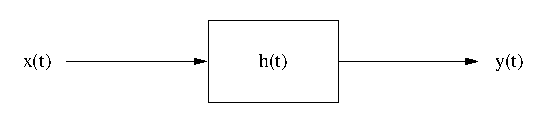
\includegraphics{simpleltisystem}
\end{center}
The implication is that in this case the signals are related by $y(t) = x(t) \conv h(t)$.  Note that the impulse response only characterises the system completely if it is LTI:  a system that is not LTI does not have an impulse response.

\subsection{Convolution}

As defined, the mathematical process of convolution takes two signals $x(t)$ and $h(t)$, and from these produces an output signal $y(t)$ according to the relation
\begin{equation*}
  y(t) = \int_{-\infty}^\infty x(\tau) h(t - \tau) d\tau.
\end{equation*}
Suppose you're given $x(t)$ and $h(t)$, and want to find the result of the convolution.  Essentially what you want is a plot of $y(t)$ versus time for all possible values of $t$.  Since $y(t)$ is just a function, we can obtain the value $y(t)$ for say $t=3$ by calculating
\begin{equation*}
  y(3) = \int_{-\infty}^\infty x(\tau) h(3 - \tau) d\tau.
\end{equation*}
In this expression $\tau$ is an integration variable that is eliminated in the integration, resulting in a {\em number} that we call $y(3)$.  This gives us one point on our $y(t)$ plot --- the value for $t=3$.  According to the formula, to find this value we need to plot $x(\tau)$ and $h(3-\tau)$ as functions of $\tau$, find the product $x(\tau) h(3-\tau)$ as a function of $\tau$, and then calculate the total area under this resulting function.  In principle to plot the whole of $y(t)$ we need to repeat this process for every value of $t$.

Suppose for example that $x(t) = p_{10}(t)$ (a centered pulse of total width 10) and $h(t) = u(t-1)$:
\begin{center}
  \psfrag{t}{\scriptsize $t$}
  \psfrag{x(t)}{\scriptsize $x(t)$}
  \psfrag{h(t)}{\scriptsize $h(t)$}
  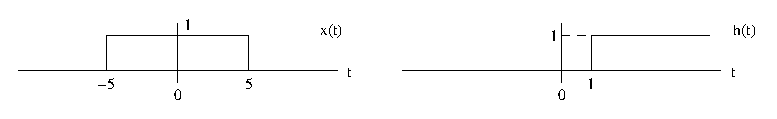
\includegraphics{convexample}
\end{center}
The required quantities for calculating $y(3)$ are 
\begin{center}
  \psfrag{tau}{\scriptsize $\tau$}
  \psfrag{x(tau)}{\scriptsize $x(\tau)$}
  \psfrag{h(3-tau)}{\scriptsize $h(3-\tau)$}
  \psfrag{x(tau)h(3-tau)}{\scriptsize $x(\tau) h(3-\tau)$}
  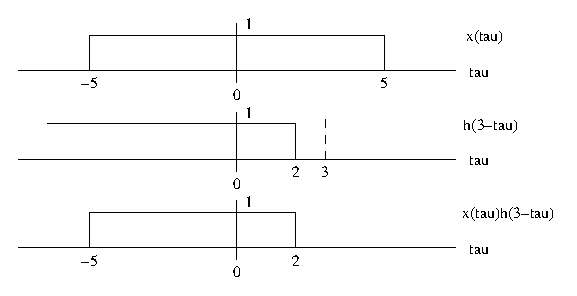
\includegraphics{convexample2}
\end{center}
Since the total area under $x(\tau) h(3-\tau)$ is 7, we conclude that $y(3) = 7$.

To find the output $y(t) = x(t) \conv h(t)$ we need to repeat the above process for all possible values of $t$.  Noting that plotting $h(t-\tau)$ as a function of $\tau$ involves a flip around the origin, and a shift of the origin to position $t$, we can generally denote it as follows:
\begin{center}
  \psfrag{tau}{\scriptsize $\tau$}
  \psfrag{h(t-tau)}{\scriptsize $h(t-\tau)$}
  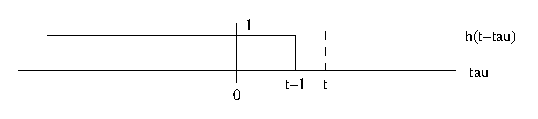
\includegraphics{convexample4}
\end{center}
In forming the product $x(\tau) h(t-\tau)$ there are three different cases to consider:
\begin{center}
  \psfrag{t}{\scriptsize $t$}
  %\psfrag{t-1}{\scriptsize $t-1$}
  \psfrag{tau}{\scriptsize $\tau$}
  \psfrag{x(tau)}{\scriptsize $x(\tau)$}
  \psfrag{h(t-tau)}{\scriptsize $h(t-\tau)$}
  \psfrag{x(tau)h(t-tau)}{\scriptsize $x(\tau) h(t-\tau)$}
  \psfrag{t-1<-5}{\scriptsize $t-1<-5$}
  \psfrag{-5<=t-1<=5}{\scriptsize $-5 \leq t-1 \leq 5$}
  \psfrag{t-1>5}{\scriptsize $t-1>5$}
  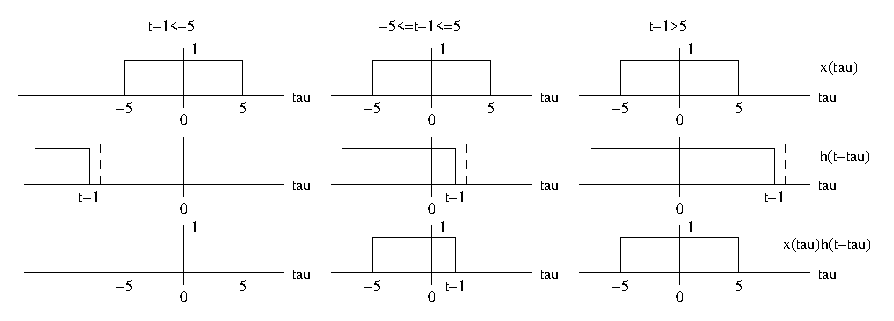
\includegraphics{convexample3}
\end{center}
For $t-1<-5$, or $t<-4$, the total area under the product is zero and $y(t)=0$ over this range.  For $-5 \leq t-1 \leq 5$, or $-4 \leq t \leq 6$ the total area under the product is $t-1+5$, so $y(t) = t+4$ over this range.  For $t-1>5$, or$t>6$, the total area is 10 and we have $y(t)=10$ in this case.  The required convolution can therefore be written in the form
\begin{equation*}
  y(t) = \begin{cases}
    0 \qquad & t<-4 \\
    t+4 \qquad & -4 \leq t \leq 6 \\
    10 \qquad & t>6,
  \end{cases}
\end{equation*}
so the output is the signal shown below:
\begin{center}
  \psfrag{t}{\scriptsize $t$}
  \psfrag{y(t)}{\scriptsize $y(t)$}
  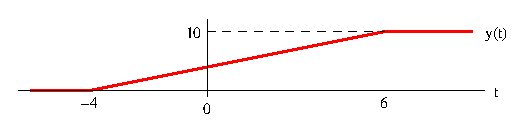
\includegraphics{convexample5}
\end{center}

For more complicated signals it may be necessary to use calculus and algebra to find the resulting output.  For example, suppose we are given the signals $x(t)$ and $h(t)$ below, and want to find $y(t) = h(t) \conv x(t)$:
\begin{center}
  \psfrag{t}{\scriptsize $t$}
  \psfrag{x(t)}{\scriptsize $x(t)$}
  \psfrag{h(t)}{\scriptsize $h(t)$}
  \psfrag{1/2}{\scriptsize $\frac{1}{2}$}
%  \psfrag{3/2}{\scriptsize $\frac{3}{2}$}
  \psfrag{e^t}{\scriptsize $e^t$}
  \psfrag{e^{-2t}}{\scriptsize $e^{-2t}$}
  \psfrag{e^{-2(t-1/2)}}{\scriptsize $e^{-2(t-\frac{1}{2})}$}
  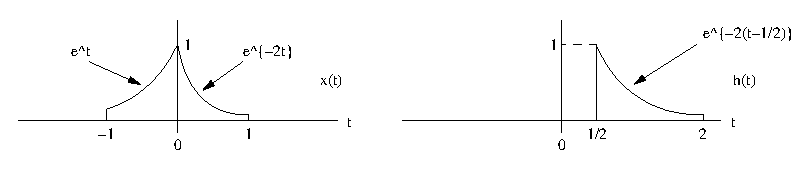
\includegraphics{convexample6}
\end{center}
We flip and shift the "easier" signal, so use the form $y(t) = \int_{-\infty}^\infty x(\tau) h(t-\tau) d\tau$.  The functions that need to be multiplied and integrated are expressed as a function of $\tau$ are as follows:
\begin{center}
  \psfrag{tau}{\scriptsize $\tau$}
  \psfrag{x(tau)}{\scriptsize $x(\tau)$}
  \psfrag{h(t-tau)}{\scriptsize $h(t-\tau)$}
  \psfrag{t}{\scriptsize $t$}
  \psfrag{t-1/2}{\scriptsize $t-\frac{1}{2}$}
  \psfrag{t-2}{\scriptsize $t-2$}
  \psfrag{e^{tau}}{\scriptsize $e^{\tau}$}
  \psfrag{e^{-2tau}}{\scriptsize $e^{-2\tau}$}
  \psfrag{e^{-2((t-tau)-1/2)}}{\scriptsize $e^{-2((t-\tau)-\frac{1}{2})}$}
  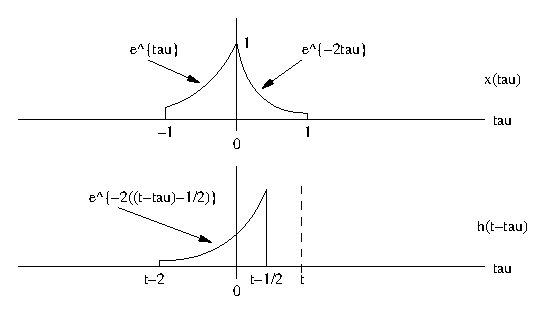
\includegraphics{convexample7}
\end{center}
As $t$ varies the function $h(t-\tau)$ changes position along the $\tau$ axis.  To find $y(t)$ we need to find the area under the product $x(\tau) h(t-\tau)$ for {\em each} value of $t$.

For simplicity, let's consider just finding the value $y(1)$.  The signals in the convolution integral are roughly as drawn above (with $t=1$), so the product is only nonzero over the range $-1$ to $1 - \frac{1}{2}$.  The required output is therefore 
\begin{align*}
  y(1) &= \int_{-1}^{\frac{1}{2}} x(\tau) h(t-\tau) d\tau 
  = \int_{-1}^0 x(\tau) h(t-\tau) d\tau + \int_0^{\frac{1}{2}} x(\tau) h(t-\tau) d\tau \\
  &= \int_{-1}^{0} e^{\tau} e^{-2((t-\tau)-\frac{1}{2})} d\tau + \int_{0}^{\frac{1}{2}} e^{-2\tau} e^{-2((t-\tau)-\frac{1}{2})} d\tau,
\end{align*}
where the integral is split into two because the signal $x(\tau)$ is defined differently over two regions of the domain.  

In general, the convolution will take the same form as above as long as $t-\frac{1}{2} \geq 0$ and $t-2 \leq -1$:  in this case the nonzero region of the product will be from $-1$ to $t-\frac{1}{2}$, with some portion of the positive $\tau$ domain included in this region.  The required convolution values will be
\begin{align*}
  y(t) &= \int_{-1}^{t-\frac{1}{2}} x(\tau) h(t-\tau) d\tau 
  = \int_{-1}^0 x(\tau) h(t-\tau) d\tau + \int_0^{t-\frac{1}{2}} x(\tau) h(t-\tau) d\tau \\
  &= \int_{-1}^{0} e^{\tau} e^{-2((t-\tau)-\frac{1}{2})} d\tau + \int_{0}^{t-\frac{1}{2}} e^{-2\tau} e^{-2((t-\tau)-\frac{1}{2})} d\tau.
\end{align*}
This gives the required output for any $\frac{1}{2} \leq t \leq 1$.

Finding the remainder of the convolution output is laborious but conceptually identical.  Critical values of $t$ are defined by the following:  $t-\frac{1}{2} = -1$, $t-\frac{1}{2} = 0$, $t-\frac{1}{2} = 1$, $t-2 = -1$, $t-2 = 0$, and $t-2 = 1$.  Ordering these critical points yields the following values of $t$:  $-\frac{1}{2}, \frac{1}{2}, 1, \frac{3}{2}, 2, 3$.  The calculation of the convolution will therefore require separate consideration of values of $t$ in intervals $(-\infty, -\frac{1}{2}]$, $[-\frac{1}{2}, \frac{1}{2}]$, $[\frac{1}{2}, 1]$, $[1, \frac{3}{2}]$, $[\frac{3}{2}, 2]$, $[2, 3]$, $[3, \infty)$.  In each case the integral will differ either in terms of the integration limits or in the specification of the integrand.

\subsection{Convolution properties}

The convolution operation has many properties, which provide insight into the operation itself as well as into the action of LTI systems on input and output signals.  A list of basic convolution properties follows:
\begin{center}
  \fbox{
    \begin{minipage}{0.9\textwidth}
      \begin{tabular}{rl}
        $x(t) \conv v(t) = v(t) \conv x(t)$ & \qquad (commutative) \\
        $x(t) \conv (v(t) \conv w(t)) = (x(t) \conv v(t)) \conv w(t)$ & \qquad (associative) \\
        $x(t) \conv (v(t) + w(t)) = x(t) \conv v(t) + x(t) \conv w(t)$ & \qquad (distributive over addition) \\
        $x(t) \conv \delta(t) = x(t)$ & \qquad (identity element) \\
        $x(t) \conv \delta(t-c) = x(t-c)$ & \qquad (shifted identity).
      \end{tabular}
    \end{minipage}
  }
\end{center}
These properties can all be derived directly from the definition of convolution.  For example, commutativity states that $x(t) \conv v(t) = v(t) \conv x(t)$ and is quite easy to prove via a change of variables (letting $p = t - \tau$ below):
\begin{equation*}
  x(t) \conv v(t) = \int_{-\infty}^\infty x(\tau) v(t - \tau) d\tau = \int_{-\infty}^\infty x(t - p) v(p) dp
  = \int_{-\infty}^\infty v(p) x(t - p) dp = v(t) \conv x(t).
\end{equation*}
Similarly, the shifted identity property follows from the sifting property:  since by definition
\begin{equation*}
  x(t) \conv v(t) = \int_{-\infty}^\infty v(\tau) x(t - \tau) d\tau,
\end{equation*}
if we let $v(t) = \delta(t - c)$ we get:
\begin{align*}
  x(t) \conv \delta(t - c) &= \int_{-\infty}^\infty \delta(\tau - c) x(t - \tau) d\tau
  = \int_{-\infty}^\infty \delta(\tau - c) x(t - c) d\tau \\
  &= x(t - c) \int_{-\infty}^\infty \delta(\tau - c) d\tau = x(t - c).
\end{align*}

Some of the properties can also be justified using basic theory for linear systems.  For example, the distributive property $x(t) \conv (v(t) + w(t)) = x(t) \conv v(t) + x(t) \conv w(t)$ is obvious if we think of a system with impulse response $x(t)$ being driven by the signal $v(t) + w(t)$:
\begin{center}
  \psfrag{x(t)}{\scriptsize $x(t)$}
  \psfrag{y(t)}{\scriptsize $y(t)$}
  \psfrag{v(t)+w(t)}{\scriptsize $v(t) + w(t)$}
  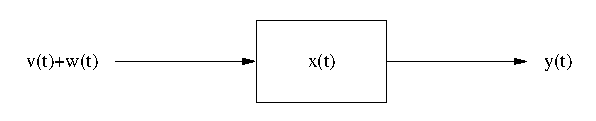
\includegraphics{simpleltisystem1}
\end{center}
The output will be $y(t) = x(t) \conv (v(t) + w(t))$.  However, we know that the following input-output pairs are valid:
\begin{align*}
  v(t) & \longrightarrow x(t) \conv v(t) \\
  w(t) & \longrightarrow x(t) \conv w(t).
\end{align*}
Since the the system is LTI we know that additivity holds, so it must also be the case that $y(t) = x(t) \conv v(t) + x(t) \conv w(t)$, and the property is seen to be true.  The identity and shifted identity properties follow similarly:  if the input is $\delta(t)$ then we know that the output must be the impulse response $x(t)$, so $x(t) \conv \delta(t) = x(t)$;  if the input is the shifted impulse $\delta(t - c)$ then the output must be the shifted impulse response $x(t - c)$, so we have $x(t) \conv \delta(t - c) = x(t - c)$.

Consider a series combination or {\em cascade} of two LTI systems, as shown below:
\begin{center}
  \psfrag{x(t)}{\scriptsize $x(t)$}
  \psfrag{y(t)}{\scriptsize $y(t)$}
  \psfrag{z(t)}{\scriptsize $z(t)$}
  \psfrag{f(t)}{\scriptsize $f(t)$}
  \psfrag{g(t)}{\scriptsize $g(t)$}
  \psfrag{h_{eff}(t)}{\scriptsize $h_{\text{eff}}(t)$}
  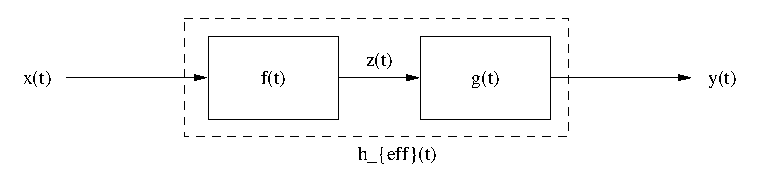
\includegraphics{lticascade}
\end{center}
Since $z(t) = f(t) \conv x(t)$ and $y(t) = g(t) \conv z(t)$, the overall input-output relation for the combined system is $y(t) = g(t) \conv (f(t) \conv x(t))$.  The associative property allows us to instead write
\begin{equation*}
  y(t) = (g(t) \conv f(t)) \conv x(t)= h_{\text{eff}}(t) \conv x(t),
\end{equation*}
where $h_{\text{eff}}(t) = g(t) \conv f(t)$ is the overall effective impulse response of the combined system.  From commutativity the effective system is exactly the same as the one below:
\begin{center}
  \psfrag{x(t)}{\scriptsize $x(t)$}
  \psfrag{y(t)}{\scriptsize $y(t)$}
  \psfrag{f(t)}{\scriptsize $f(t)$}
  \psfrag{g(t)}{\scriptsize $g(t)$}
  \psfrag{h_{eff}(t)}{\scriptsize $h_{\text{eff}}(t)$}
  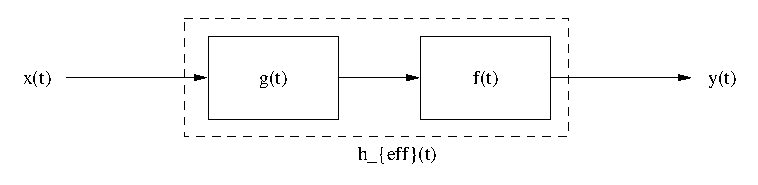
\includegraphics{lticascade2}
\end{center}
Thus the order of LTI systems arranged in a series combination can be changed without affecting the overall system response.

Other properties can also be derived that relate inputs and outputs of a convolution.  Assuming that $y(t) = x(t) \conv v(t)$, the following are also true:
\begin{center}
  \fbox{
    \begin{minipage}{0.9\textwidth}  
      \begin{tabular}{rl}
        $y(t-c) = x(t-c) \conv v(t) = x(t) \conv v(t-c)$ & \qquad (shifting) \\
        $\frac{d}{dt} y(t) = \frac{d}{dt} x(t) \conv v(t) = x(t) \conv  \frac{d}{dt} v(t)$ & \qquad (derivative) \\
        $\int_{-\infty}^t y(\tau) d\tau = \int_{-\infty}^t x(\tau) d\tau \conv v(t) = x(t) \conv  \int_{-\infty}^t v(\tau) d\tau$ & \qquad (integration).
      \end{tabular}
    \end{minipage}
  }
\end{center}
The derivative property can be obtained directly from the definition
\begin{equation*}
  y(t) = x(t) \conv v(t) = \int_{-\infty}^\infty x(\tau) v(t - \tau) d\tau.
\end{equation*}
Taking the derivative with respect to time on both sides gives
\begin{equation*}
  \frac{d}{dt} y(t) = \frac{d}{dt} \left\{ \int_{-\infty}^\infty x(\tau) v(t - \tau) d\tau \right\}
  = \int_{-\infty}^\infty x(\tau) \left\{ \frac{d}{dt} v(t - \tau) \right\} d\tau
  = \int_{-\infty}^\infty x(\tau) \dot{v}(t - \tau) d\tau,
\end{equation*}
so $\dot{y}(t) = x(t) \conv \dot{v}(t)$ (where the dot above the signal indicates the generalised time derivative).  One form of the shifting property follows again from the interpretation of $y(t) = x(t) \conv v(t)$ as the input-output relation for a system with impulse response $x(t)$ driven by the signal $v(t)$.  Since the system is time invariant (or it wouldn't have an impulse response and convolution would be meaningless), the response to the shifted input $v(t-c)$ must be $y(t-c)$ and it must always be true that $y(t-c) = x(t) \conv v(t-c)$.

The integration property can be justified using basic properties of LTI systems.  Consider the cascade below:
\begin{center}
  \psfrag{x(t)}{\scriptsize $x(t)$}
  \psfrag{y(t)}{\scriptsize $y(t)$}
  \psfrag{v(t)}{\scriptsize $v(t)$}
  \psfrag{g(t)}{\scriptsize $g(t)$}
  \psfrag{w(t)}{\scriptsize $w(t)$}
  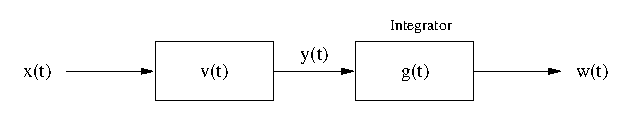
\includegraphics{integrationcascade2}
\end{center}
The input-output relation for the integrator is $w(t) = \int_{-\infty}^t y(\tau) d\tau$, which can be shown to satisfy the requirements for linearity and time invariance.  (The system therefore does have an impulse response $g(t)$, but we're not making use of this fact here.)  Also, $y(t) = v(t) \conv x(t)$. 

Since both component systems are LTI, from an overall input-output perspective the combined system above is equivalent to
\begin{center}
  \psfrag{x(t)}{\scriptsize $x(t)$}
  \psfrag{y(t)}{\scriptsize $y(t)$}
  \psfrag{v(t)}{\scriptsize $v(t)$}
  \psfrag{g(t)}{\scriptsize $g(t)$}
  \psfrag{z(t)}{\scriptsize $z(t)$}
  \psfrag{w(t)}{\scriptsize $w(t)$}
  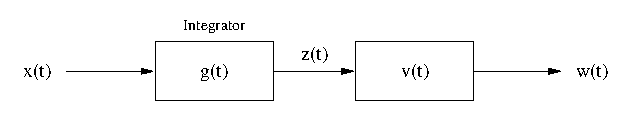
\includegraphics{integrationcascade}
\end{center}
In this case
\begin{equation*}
  w(t) = v(t) \conv z(t) = v(t) \conv \int_{-\infty}^t x(\tau) d\tau.
\end{equation*}
For the same input $x(t)$ the output $w(t)$ must be the same for both cases shown, so we must have
\begin{equation*}
  \int_{-\infty}^t y(\tau) d\tau = v(t) \conv \int_{-\infty}^t x(\tau) d\tau
\end{equation*}
as long as $y(t) = v(t) \conv x(t)$.

{\em The\marginpar{\bf Exercise:} integrator system (also called an accumulator) has an impulse response $g(t) = u(t)$.  Assume this to be true and use the definition of convolution to show that the system has the required input-output relation.}

\subsection{Example:  smoothing a rectangular pulse train}

\end{document} 

